\subsubsection{\theoryC{Prospects for Boosted Object Tagging with Timing Layers}}
\label{sec:theoryboostedtiming}
\contributors{Matthew D. Klimek}
%\textbf{Authors: Matthew D. Klimek$^{a,b}$}\\
%\textit{a) Laboratory for Elementary Particle Physics, Cornell University, Ithaca, NY 14853, USA
%b) Department of Physics, Korea University, Seoul 02841, Republic of Korea
%}\\
%\texttt{klimek@cornell.edu}

Both CMS and ATLAS are studying new timing detectors to be installed for the high luminosity phase of the LHC. 
The primary motivation for these new detectors is to aid in mitigating the increased level of pileup that comes along with the increased luminosity.
The $\mathcal O$(30 ps) timing resolution will permit individual proton-proton interactions within a single bunch crossing to be temporally resolved.
Beyond pileup mitigation, these detectors may be useful for novel kinds of searches.
For example, it has been proposed in \citeref{Liu:2018wte} that they could be used to set limits on long-lived particles.
In this section, we point out that this level of timing precision provides the capability of temporally resolving jets for the first time.
Currently, jet substructure techniques play a major role in the search for BSM physics.
These exploit correlations in momentum and angular distribution of jet constituents to distinguish standard QCD jets from other objects.
The capabilities of the new timing layers open up the possibility of extending jet substructure techniques to the time domain.
In this section, we will introduce the relevant concepts and suggest that time domain jet substructure can play a complementary role to existing techniques in the search of boosted resonances at the HL-LHC.

Of the various physics objects that are reconstructed by the LHC experiments, jets are unique in that they are collections of particles.
The individual jet constituents have some spread in velocity and therefore arrive at the detector over some finite span of time.
On dimensional grounds, we can estimate that the typical scale of Lorentz boosts of the jet constituents is $\gamma = E/m \sim E_j/n\Lambda_\mathrm{QCD}$, where $E_j$ is the jet energy, $n$ is the hadron multiplicity of the jet, and $\Lambda_\mathrm{QCD}$ sets the typical hadron mass.
The corresponding scale of the spread in arrival times at a detector a distance $R$ from the interaction point is then of order $\delta t\sim R\delta v\sim R\gamma^{-2}$. 
For $R\sim$~1 m, $E_j\sim$~100 GeV, $n\sim$~10, and $\Lambda_\mathrm{QCD}~\sim$~1 GeV, we have $\delta t\sim$~100 ps.
Thus we see that at typical LHC energies, the proposed timing detectors with $\mathcal O$(30 ps) resolution should be sensitive to the temporal structure of jets.

We note that this effect is entirely due to the hadronization process.
Any time differences inherent to the perturbative parton shower should be of order $\Lambda_\mathrm{QCD}^{-1}$ and will be far below the resolution of the timing detectors.
(In practice, the distance from the interaction point to the timing detector will have some dependence on pseudorapidity $\eta$.
Because the showering process produces radiation in a cone around the original parton direction, the various jet constituents will then have slightly different distances to travel to the detector.
However, for reasonably central jets, this will be a small effect.)
If, in the hadronization process, jet constituents are produced with rapidities $y$ distributed according to $dN/dy = f(y)$, then it is easy to verify that at a detector a distance $R$ in any direction from the interaction point, they will arrive distributed in time according to 
\begin{equation}
	\frac{dN}{dt} = \frac{ cR f(y(t)) }{ (ct)^2-R^2},
\end{equation}
with $ct>R$, where $c$ is the speed of light and $y(t)=\mathrm{arctanh}(R/ct)$.
Although it is not possible to calculate $f(y)$ from first principles, we note that for any reasonably well-behaved $f(y)$ the arrival time distribution will indicate a burst of jet constituents arriving promptly with a tail extending out to later times.

The hadronization process is treated phenomenologically by a number of models, and we can verify that this behavior is borne out.
For example, the simplest form of the Lund string hadronization model~\cite{Andersson:1983ia} predicts $f(y)=$~constant.
PYTHIA implements a more complete version of the Lund model, and we use it to verify the predictions of the preceding paragraphs.
We generated a sample of 50 GeV quark jets from $e^+e^-$ annihilation in PYTHIA8, and computed the arrival times of all charged hadrons in each jet at a distance of 1 meter from the interaction point.
A histogram with 100 ps bin size of the averaged arrival time profile is shown in Figure~\ref{fig:pythia_arrival_profile}.
We can see that the PYTHIA output displays the expected behavior, and we verify that the typical width of the profile is indeed $\mathcal O(100)$~ps.

\begin{figure}
	\begin{center}
		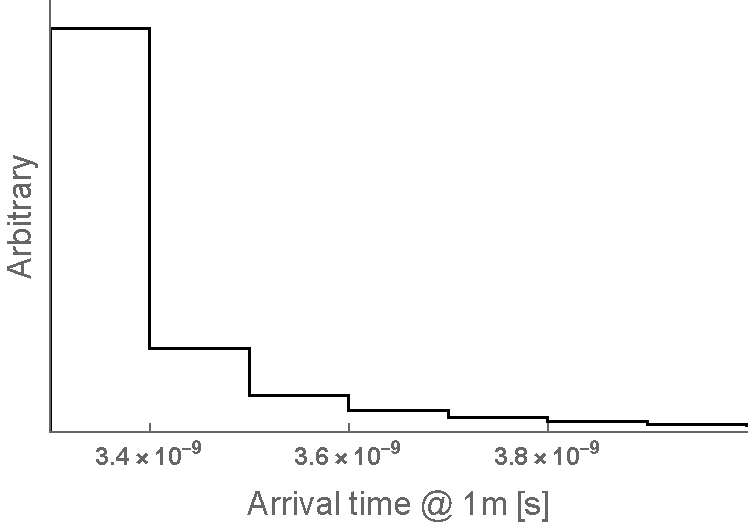
\includegraphics[width=0.4 \linewidth]{\main/section7OtherSignatures/img/arrival_time_profile.pdf}
	\end{center}
	\caption{Average arrival time profile at 1 meter for charged hadrons in 50 GeV quark jets from $e^+e^-$ annihilation as simulated by PYTHIA8.}
\label{fig:pythia_arrival_profile} 
\end{figure}

A study of the rapidity distribution of jet constituents from arrival time profile of QCD jets could provide additional data with which to tune our models of hadronization.
However, we will now argue that this information also provides a novel method for distinguishing normal QCD jets from jets produced by boosted objects.
As described in the preceding paragraphs, in a typical jet we expect most hadrons to arrive together and a few to arrive at later times.
Note that under a boost, the ordering of the jet constituents in velocity or rapidity is unchanged.
Consider a massive particle that decays in its rest frame producing a jet pointing along the negative $x$ axis.
The particles in the tail of its velocity distribution have velocities along the $x$ direction that are less negative than the rest of the jet.
Now consider the same massive particle but with a large boost in the positive $x$ direction so that this jet is boosted forward into the positive direction as well.
Despite the change in direction, the ordering of the velocities in the jet is the same.
The velocities of all jet constituents are now positive, and the tail of the distribution is more positive.
We see that if a jet is sufficiently boosted, the tail of its hadron distribution can arrive at the detector first.

In order to quantify this effect, we make use of a simple diagnostic that can distinguish the boosted from the unboosted jets based on their arrival time profiles.
Recall that for an unboosted jet, we expect the majority of the charged hadrons to arrive in close temporal proximity with a few arriving later, whereas for a sufficiently boosted jet, one or more charged hadrons may arrive before most of the others.
Let $t_i$ and $p_{i}$ be the arrival times and momenta of the charged hadrons in a jet and $\bar t$ be the median charged hadron arrival time.
We define the diagnostic function
\begin{equation}
	D_\tau = \frac{ \sum p_{i} \Theta(t_i-\bar t-\tau) }{ \sum p_{i} }.
\end{equation}
The parameter $\tau$ should be a value of order the time resolution of the detector.
For an unboosted jet, the median arrival time will be in the prompt burst of hadrons.
For an appropriate value of $\tau$, none of these hadrons nor any that arrive later will satisfy the theta function, and we will obtain $D_\tau=0$.
However, for boosted jets, some hadrons from the boosted tail may arrive before the main burst. Because the median will still be in the main burst, the early hadrons can satisfy the theta function, in which case we will find $D_\tau>0$.

To verify this behavior, we generate two samples of jets in PYTHIA8.
The first is a sample of 500 GeV quark jets from $e^+e^-$ annihilation.
For comparison, we also generate a similar sample of 50 GeV jets, but then boost them by $v=0.98$.
This is comparable to jets that would be observed from $Z$ decay, where the $Z$ has been produced in the decay of a 1 TeV diboson resonance.
We choose a conservative value of $\tau=200$~ps, which is several times the expected timing detector resolution.
In the first sample, we find that our diagnostic is zero in all but 1\% of events.
However, for the boosted jet sample, we obtain non-zero values in 25\% of events.

The actual operating environment of the HL-LHC will present additional challenges coming from the noisy hadronic environment.
Jet contamination from pileup and underlying event radiation could mimic the early arrival of the tail of a boosted jet.
The information from the timing layers will be used to mitigate pileup and jet grooming techniques can be used to remove stray radiation from the jets before their temporal characteristic are analyzed.
The timing substructure information can then be combined with existing jet substructure techniques to increase the efficiency for tagging boosted objects, in turn improving the reach of BSM searches.
During an HL-LHC phase, even higher boosts can be expected, demanding effective techniques for boosted object tagging.
Further details are presented in \citeref{Klimek:inprep}.
